\chapter{GitHub Actions}

GitHub Actions是由著名代码托管平台GitHub推出的持续集成和持续部署工具,
于2020年提供于所有GitHub用户使用。除了开源代码库可以免费使用该功能外,
还为每个账户提供了每月多达2000分钟的私有仓库运行时间。同时,
GitHub Actions还同时支持Windows、Linux、MacOS环境,提供流水线功能,
支持并发集成和测试,快速引用其他人编写的集成工具等,是一个功能强大的工具。

GitHub Actions目前只支持托管于GitHub上的仓库使用。一个仓库使用GitHub
Actions需要在.github/workflows/中新建定义一个Action的yml文件,
一个仓库可以有多个Action文件,用于不同任务。

\begin{figure}
    \centering
    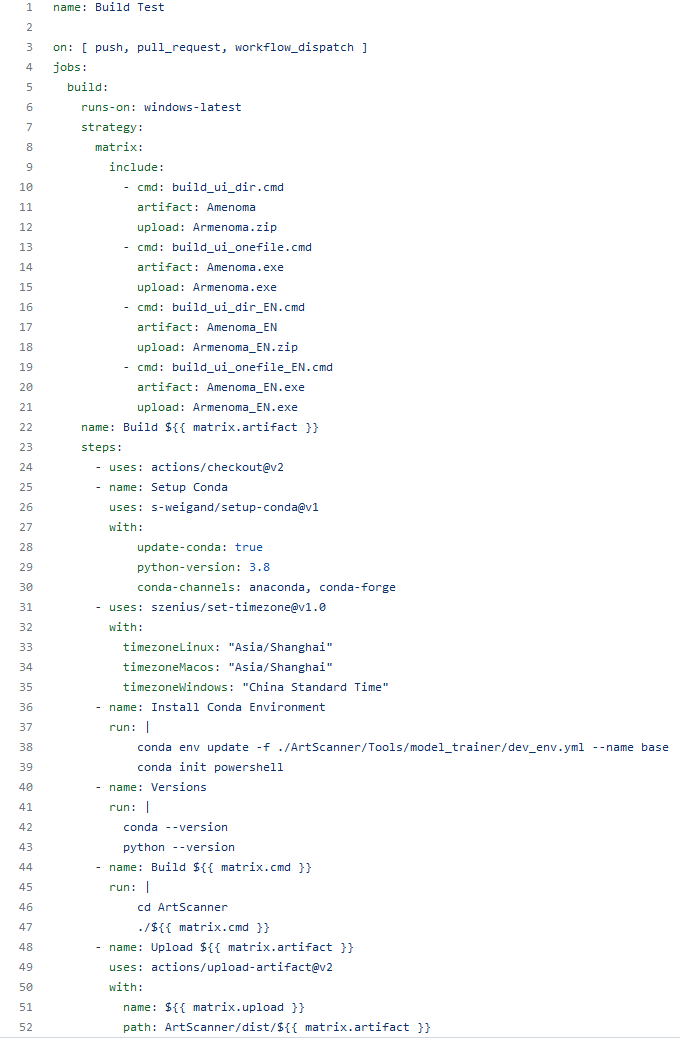
\includegraphics[width=1\textwidth]{figures/github/actions.png}
    \caption{GitHub Actions}
    \label{fig:githubactions}
\end{figure}

图\ref{fig:githubactions}给出了一份GitHub Actions配置。

第1行定义了工作流的名称,第3行定义了工作流的触发条件。接下来定义了不同的jobs,
本例中只包含一个build的job,在一些大型项目中,可以包含编译、测试、打包等不同的job,
且不同的job之间可以进行文件传递,且可以指定依赖关系,因此可以完成交叉编译等复杂任务。

第7-21行是GitHub Actions的策略矩阵功能,可以同时启动多个实例执行较为相似的任务。
在本例中,由于产物包含中文、英文、可执行文件和压缩包共四种组合产物,其持续集成代码接近,
通过策略矩阵,可以同时编译四种产物,大大减少编译时间的同时还减轻了工作流编写的代码量。
策略矩阵也被常用于同时执行大量单元测试。

在第24、26、31、49行,引用了其他人编写的配置,这是GitHub Actions的一个特色,
这些配置均为GitHub中的一个仓库,这种方式大大提高了Actions的灵活性和可复用性。
在本例中,引用的配置分别用于自动从GitHub拉取代码,激活conda环境,设置时区,
以及上传集成后产物。

第37-47行为执行脚本,GitHub Actions基于容器实现,在执行时内部环境和普通服务器无异,
因此可以很方便的进行复杂配置。

在本例中配置并未包含流水线和持续部署相关的代码,实际上GitHub Actions均可以实现。
对于流水线,只需要启动多个jobs,例如build/test/deploy并指定依赖关系,
就可以做到流水线作业。而对于持续部署,GitHub仓库中可以设定Actions执行时
可以使用的隐私信息,通过将SSH私钥或服务器密码等设置为隐私信息,
服务器可以在持续集成完成后通过密钥访问部署服务器并进行自动部署。
然而,作为一个提供公开服务且位于国外的公司,这样做的安全性较低,
仅作为小规模、低成本、个人服务器部署的可选方案,例如利用Actions对静态网页自动
编译,并将编译结果上传至博客服务器等。